\section{Introduction}

%\subsection{Problem Statement \redtext{(what is the problem to be solved?)}}
%We develop a centralized method for estimating missing data in sensor network datasets, a procedure which is crucial for subsequent analysis.
%Missing data imputation (a term from Statistics) has a long history, and while there are many existing algorithms which estimate missing sensor data (as documented in Section \ref{sec:rw}), few of these take advantage of the time and inter-sensor correlations inherent in the WSN datasets.
%Furthermore, distributed approaches~\cite{xiao2006space,nowak2003distributed} are often limited to providing estimations or decisions based on sensors in the immediate neighborhood and rely on the deployed sensors having adequate computational power to perform such calculations.
%Not suffering from these issues, the centralized approach we have taken enables a global solution (utilizing all observations available from the sensor network) and provides a vital backdrop for our novel highly-accurate sensor network data imputation technique.

%\subsection{Relevance (why is WSN dataset analysis an important topic?)}
%The increasing pervasiveness of Wireless Sensor Network (WSN) deployments is reflected by the recent coinage of terms such as ``Internet of Things'' and ``Machine-to-Machine'' to describe this growing revolution~\cite{ashton2009internet,gershenfeld2004internet,nokia2004machine,lawton2004machine}.
%Facilitated by a sharp reduction in hardware costs~\cite{estrin2000special}, this growing trend (beyond providing for the admission of new phrases into the vernacular) has led to an explosion in the amount and variety of sensor network todata in need of study.
%For this reason, analysis of WSN data has garnered much attention in recent years~\cite{balazinska2007data}.

%\subsection{Motivation \redtext{(why is data imputation needed for WSN datasets?)}}

% Data sets gathered from sensor networks often suffer from a significant fraction of missing data, due to issues such as 
% communication interference, sensor interference, power depletion, and hardware failure. 
% Many standard data analysis tools such as classification engines, time-sequence pattern analysis modules, and even statistical tools are ill-equipped to deal will missing values---hence, there is a need to impute missing readings prior to analysis.

Wireless sensor networks (WSNs) are especially susceptible to interference,
battery depletion, hardware failures, and other environmental and communications ailments
that lead to data loss.  Datasets gathered from sensor networks\footnote{We consider the common setting where sensor readings are collected in order to perform centralized analysis.}
 are
often missing a significant fraction of the possible readings
(e.g., the Intel Berkeley Research lab dataset~\cite{berkeley2004lab}
is missing roughly 50\%).
These missing values are problematic for data analysis tools such as
classification engines, time-sequence pattern analysis modules, and
other machine learning tasks, which are often ill-equipped to deal
with missing values.  Support Vector Machine (SVM)
%~\cite{vapnik2000nature} 
and Multiple Regression (MR) analysis,
to name but a few examples, require complete datasets with no missing
values.  Popular statistical packages such as SAS, Stata, and R
provide a few default options for handling missing data, as a
preprocessing step, because the core algorithms require that all data be filled
in.  Typical options are (i) remove the entire ``column'' if there is a
missing value or (ii) fill in the missing value (called {\em
imputation}) using either simple defaults like the average of
neighboring values or utilizing user-written code.  
The first option discards
otherwise useful data, and in fact, may discard most of the columns in
datasets with high data loss.  
Thus, imputation is a vital tool in the
preparation of sensor data for subsequent analysis. 
Because the
accuracy of the target data analysis depends on the accuracy of the
imputation, improvements in sensor data imputation better serve
sensor network deployment objectives.

%We consider the common setting where the goal is to collect all the sensor readings
%in order to perform centralized analysis, while maximizing the lifetime of the WSN.
%Sensor nodes are battery powered and may be energy-harvesting, and will often make
%only a ``best effort'' attempt to transmit their readings back to the centralized 
%collection point.  This contributes to the prevalence of missing data, furthering
%the value of effective imputation techniques.

%\subsection{Background \redtext{(what solutions currently exist?)}}

%\subsection{Method Overview \redtext{(what is our approach to bridge the research gap?)}}

\subsection{Our Approach: Collaborative Filtering}

\vspace{-0.5cm}

\begin{figure}[h]
\centering

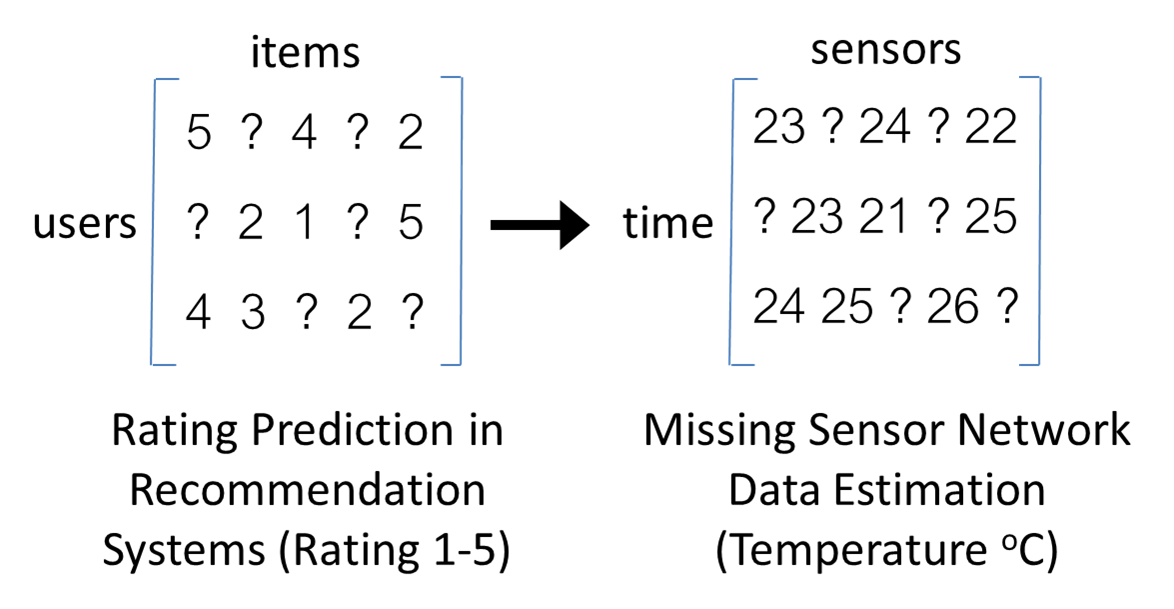
\includegraphics[scale=0.30,trim=4 4 4 4,clip]{recommend_imputation_timerow_white.eps}
\vspace{-0.1in}
\caption{Bridge from Recommendation Systems to Sensor Data Imputation} 
\label{recommend_imputation}
\vspace{-0.1in}
\end{figure}

Unlike prior work in sensor data imputation~\cite{Granger:lastseen, le2005estimating, 
Gruenwald:FARM, li2008data, yuan2000multiple, Jian-Zhong:STI, pan2010k,
osborne2012real, beckers2003eof, kondrashov2006spatio}, this paper presents a {\em Collaborative Filtering} (CF) 
approach to sensor data imputation, inspired by the field of Recommendation
Systems.  In typical CF approaches, the elements of interest are users
and items (e.g., products), and the values are user ratings of those
items (as in the left-hand side of
Figure~\ref{recommend_imputation}).  Typically, most of the ratings
are missing, and the goal is to predict (impute) the missing ratings
in order to ``recommend'' items to users.  By viewing sensors as
items, users as time steps, and readings as ratings (as illustrated in
Figure~\ref{recommend_imputation}), we can apply CF
techniques to perform sensor data imputation. 
%(Alternatively, sensors
%can be viewed as users and items as time steps---the mapping is
%irrelevant to the CF formulation.)  
In particular, we focus on the
widely successful {\em Matrix Factorization} (MF) technique for CF.

Sensor readings differ from user ratings, however, in that the former
often exhibit high correlation in both time and space.
To incorporate this property, we first modify MF
to model temporal correlations and learn latent relationships among
sensors.  Specifically, we add temporal-proximity terms to
MF---we call this {\em Temporally-Regularized MF} (TR-MF)
---to reflect the fact that readings in neighboring time steps are similar.
Similarly, we can also add spatial-proximity terms---we 
call this {\em Spatially-Temporally-Regularized} MF (STR-MF).
Second, we consider sensor networks with multiple sensor types at each node.
We are readily able to exploit such heterogeneous sensor information in our
solution, in contrast to most prior imputation methods that use more ad hoc means.
%Our method incorporates these heterogeneous sensor
%signals (for example, estimating the temperature at a given sensor
%node utilizing the humidity and temperature trends from other
%sensors in the network) to provide more accurate imputation than 
%prior approaches.
We present two techniques for extending 
TR-MF to account for possible correlations among sensor types: {\em Multivariate-TR-MF} and 
{\em Temporally-Regularized Tensor Factorization} (TR-TF).

We evaluate our approaches using two environmental sensor network
datasets, one indoor and one outdoor.
%Both datasets record temperature, humidity, and light within its deployed
%environment.  Each dataset has a roughly 50\% initial missing rate (strengthening
%the claim that missing data in WSNs is a common issue), to which we
%additionally cover known observations to use for validation and
%testing purposes.
We study two patterns for missing data: (i) covering
{\em random} readings (modeling intermittent reading failures) and (ii)
covering {\em consecutive} readings for some sensor nodes
(modeling long temporal gaps such as with failed sensors).
Our study shows that TR-MF provides significantly higher estimation accuracy than 
both (i) state-of-the-art recommendation models and (ii) state-of-the-art sensor data imputation approaches 
(discussed in Section~\ref{sec:rw}).
%AKE (which is the most accurate prior spatio-temporal method).
Furthermore, our study shows that STR-MF, which adds spatial
coordinate information into TR-MF, is useful {\em only} in the
``consecutive'' pattern---perhaps surprisingly, STR-MF is
significantly {\em less} accurate than TR-MF in the ``random''
pattern.  This is because TR-MF effectively learns the latent
relationships among sensors from data, including any spatial correlations, while
avoiding the pitfalls of spatial-proximity biases (Section~\ref{subsec:sm}).
For the heterogeneous setting, our study shows that both
Multivariate-TR-MF and TR-TF can significantly improve the accuracy over TR-MF,
and each has its strengths, depending on the observed variance in the
readings.  Finally, we consider a popular data analysis task---building regression-based prediction models---and show that,
compared to prior approaches for imputation, using TR-MF leads to a much higher quality prediction model.

%These results validate our novel approach of equating sensor imputation with recommendation systems.  
%CF approaches such as Matrix Factorization and Tensor Factorization are adept at handling scenarios 
%with large numbers of missing values.
Here we proposed a data-driven imputation model that
correlations are captured by grouping correlated sensor nodes and correlated time
steps---unlike prior sensor data imputation approaches, our CF
approaches use this {\em latent} information to impute values, and optimize the evaluation metrics directly. 
Moreover, our CF approaches are global, taking into account all
collected observations, and not overly tied to spatial-proximity
correlations.  
%For example, they can capture the correlations between
%distant sensors $3$ \& $4$ in Figure~\ref{house_floorplan}, while
%grouping sensors $1$, $2$ \& $5$ only if the observed readings warrant
%it.  The CF framework also provides a unified approach to incorporate
%any number of additional sensor types for an even more accurate imputation.

%The reason we believe our method outperforms the results of other methods are as follows.
%\begin{itemize}
%\item A CF approach utilizes {\em latent} information between sensors, e.g., inter-sensor correlation
%\item utilizing heterogeneous sensor information (e.g., utilizing humidity information when estimating temperature) provides additional features which enables a more refined estimation model
%\item we provide an efficient optimization method to learn the inherent model parameters effectively
%\item our method provides a global solution, where all sensor observations available in the dataset can potentially aid in the estimation of a given missing observation
%\end{itemize}

% Given these experimental conditions, we show that our temporal and spatial-oriented collaborative filtering approach to data imputation for WSNs performs more accurately than existing methods such as linear regression and hybrid-kNN.
% In Matrix Factorization, we impose the temporal regularization and Temporal-Regularied MF show the best performance compared to all competitor algorithmss.
% On top of that, we add in spatial regularization and multivariate learning, and we discuss under which circumstance these two are applicable and how they can even improve our models.
% We propose the Tensor Factorization model for missing data recovery. The TF model use additional dimension to capture the correlations of features such as temporal, spatial or heterogeneous signal correlations. The conventional Tensor decomposition technology can only apply on dense tensor. The study of Tensor Factorization model in Collaborative Filtering for recommendation recently, but not practical in sensor network. We  have adapted the TF model for missing value estimation. 

\subsection{Contributions}

In summary, the main contributions of this paper are:
\begin{itemize}
\item We propose viewing sensor data imputation as a recommendation problem, and modify state-of-the-art CF methods of recommendation systems as the solution. 
\item We augment collaborative filtering with temporal regularization and multi-sensor signals, and provide efficient optimization methods to learn the inherent model parameters effectively.
\item We present an empirical study on two sensor datasets, considering two
missing data patterns corresponding to intermittent readings and failed
sensors. The results show 
superior estimation accuracy,
%that our proposed approaches provide
%significantly higher estimation accuracy than state-of-the-art prior
%approaches, 
and moreover, such accuracy improvements can result in the
generation of higher-quality prediction models.
\end{itemize}

% which finds that our method works well without the incorporation spatial information and that our approach can facilitate the generation of better prediction models

%\subsection{Paper Organization}

%\noindent{\bf Roadmap.}
%%The remainder of our paper is organized as follows.  
%Related work is reviewed in Section~\ref{sec:rw}.  In Sections~\ref{sec:mf} and~\ref{sec:tf} 
%we describe our factorization and multivariate factorization
%approaches to sensor data imputation, respectively. Section \ref{sec:exp} presents our experimental study. 
%Sections \ref{sec:disc} and \ref{sec:conc} provide discussions of our findings and conclusions.
